\chapter{Programmation différentiables}\label{ch:kotlingrad}

\setlength{\epigraphwidth}{0.86\textwidth}
\epigraph{Bien que la notation mathématique possède sans aucun doute des règles d'analyse, celles-ci sont assez lâches, parfois contradictoires et rarement clairement énoncées. En raison de leur application à un large éventail de sujets, de leur grammaire stricte et de leur interprétation stricte, les langages de programmation peuvent apporter de nouvelles idées sur la notation mathématique. ''}{\begin{flushright}--Kenneth \citet{iverson1999math}, \href{https://www.cs.trinity.edu/About/The_Courses/cs301/math-for-the-layman/}{\textit{Math pour la Layman}}\end{flushright}}

Dans ce chapitre, nous aborderons la théorie et la mise en œuvre d'un langage spécifique à un domaine et sans danger pour les types, destiné à la différentiation automatique (AD), un algorithme ayant diverses applications dans l'optimisation numérique et l'apprentissage automatique. L'idée clé de l'AD est assez simple. Un petit ensemble d'opérations mathématiques primitives constitue la base de tous les ordinateurs modernes, et en composant ces opérations sur les nombres réels de manière ordonnée, on peut calculer n'importe quelle fonction calculable. Dans l'apprentissage automatique, on nous donne souvent une fonction calculable sous la forme d'un programme qui ne fonctionne pas correctement. Nous voudrions un algorithme pour déterminer comment modifier légèrement l'entrée, afin de produire une sortie plus appropriée.

Un tel algorithme a d'abord été conçu par ~\citet{wengert1964simple}, dont la méthode est connue aujourd'hui sous le nom de AD en mode avancé. Peu de temps après, un certain Richard Bellman a reproduit l'algorithme de Wengert pour estimer numériquement la dynamique orbitale d'un système à deux corps, reconnaissant son potentiel pour, "le traitement de grands systèmes d'équations différentielles qui ne pourraient pas être entrepris autrement" "~\citep{bellman1965wengert}. C'est à peu près à la même époque qu'apparurent les principaux détails de l'algorithme de rétropropagation~\citep{dreyfus1990artificial}. C'est dans la~\citet{linnainmaa1970representation} que l'idée de calculer des dérivées sur des graphiques de calcul a été enregistrée pour la première fois. L'algorithme de Linnaimaa était particulièrement important pour les réseaux de neurones, et est aujourd'hui connu sous le nom de AD en mode inverse. Mais ce n'est qu'en 2010 que les outils logiciels standard~\citep{bergstra2010theano} pour l'AD sont devenus largement disponibles dans l'apprentissage automatique. C'est ici que commence notre voyage.

\section{Différentiation automatique}\label{sec:automatic-differentiation}

Lorsqu'une fonction est dotée d'une certaine entrée, AD nous indique comment modifier l'entrée d'un montant minimal, afin de modifier les sorties au maximum. Supposons qu'on nous donne une fonction $P_k : \mathbb{R}\rightarrow\mathbb{R}$, composée d'une série de fonctions imbriquées, chacune de même type:
%
\begin{equation}
    P_k(x) = \begin{cases} p_1 \circ x = x &\text{if } k=1\\ p_k\circ P_{k-1} \circ x&\text{si } k > 1 \end{cases}
\end{equation}
%
De la règle de la chaîne, on rappelle que le dérivé d'une composition est un produit des dérivés:
%
\begin{equation} \label{eq:sfun_chain_rule}
\frac{dP}{dp_1} = \frac{dp_k}{dp_{k-1}}\frac{dp_{k-1}}{dp_{k-2}}\dots\frac{dp_2}{dp_1}= {\displaystyle \prod_{i=1}^{k-1} \frac{dp_{i+1}}{dp_{i}}}
\end{equation}
%
Étant donné $Q(q_1, \dots, q_m) : \mathbb{R}^m\rightarrow\mathbb{R}$, le \textit{gradient} est une fonction $\nabla Q : \mathbb{R}^m\rightarrow\mathbb{R}\rightarrow\mathbb{R}^m$ définie comme:
%
\begin{equation}
    \nabla Q = \left[ \frac{\partial Q}{\partial q_1}, \dots, \frac{\partial Q}{\partial q_m}\right]
\end{equation}
%
Le \textit{Hessien} est une fonction $\mathbf{H}:\mathbb{R}^m\rightarrow\mathbb{R}\rightarrow\mathbb{R}^{m\times m}$ renvoyant une matrice de partiels de second ordre:
%
\begin{equation}
    \mathbf{H}(Q) = \begin{bmatrix}{\dfrac {\partial ^{2}Q}{\partial x_{1}^{2}}}&{\dfrac {\partial ^{2}Q}{\partial x_{1}\,\partial x_{2}}}&\cdots &{\dfrac {\partial ^{2}Q}{\partial x_{1}\,\partial x_{m}}}\\[2.2ex]{\dfrac {\partial ^{2}Q}{\partial x_{2}\,\partial x_{1}}}&{\dfrac {\partial ^{2}Q}{\partial x_{2}^{2}}}&\cdots &{\dfrac {\partial ^{2}Q}{\partial x_{2}\,\partial x_{m}}}\\[2.2ex]\vdots &\vdots &\ddots &\vdots \\[2.2ex]{\dfrac {\partial ^{2}Q}{\partial x_{m}\,\partial x_{1}}}&{\dfrac {\partial ^{2}Q}{\partial x_{m}\,\partial x_{2}}}&\cdots &{\dfrac {\partial ^{2}Q}{\partial x_{m}^{2}}}\end{bmatrix}
\end{equation}
%
Pour les fonctions vectorielles $\mathbf{f} : \mathbb{R}^m\rightarrow\mathbb{R}^n$, le \textit{Jacobien}, $\mathcal{J}_{\mathbf{f}} : \mathbb{R}^m\rightarrow\mathbb{R}^n\fourchette droite\mathbb{R}^{n \times m}$ est défini comme:
%
\begin{equation}
    \mathcal{J}_{\mathbf{f}} =
    \begin{bmatrix}
        \dfrac{\partial \mathbf{f}}{\partial x_1} & \cdots & \dfrac{\partial \mathbf{f}}{\partial x_m}
    \end{bmatrix} =
    \begin{bmatrix}
        \dfrac{\partial f_1}{\partial x_1} & \cdots & \dfrac{\partial f_1}{\partial x_m}\\
        \vdots & \ddots & \vdots\\
        \dfrac{\partial f_n}{\partial x_1} & \cdots & \dfrac{\partial f_n}{\partial x_m}
    \end{bmatrix} =
    \begin{bmatrix}
        \nabla f_1 \\
        \vdots \\
        \nabla f_m
    \end{bmatrix}
\end{equation}
%
Pour les fonctions scalaires, la transposition du Hessien est équivalente au Jacobien du gradient:
%
\begin{equation}
    \mathbf{H}(Q)^\intercal = \mathcal{J}_\mathbf{q}(\nabla Q)
\end{equation}
%
Pour une fonction vectorielle $\mathbf{P}_k(\mathbf{x}) : \mathbb{R}^m\rightarrow\mathbb{R}^n$, la règle de la chaîne de \autoref{eq:sfun_chain_rule} s'applique toujours:
%
\begin{equation} \label{eq:vfun_chain_rule}
\mathcal{J}_\mathbf{P_k} = \displaystyle \prod_{i=1}^{k} \mathcal{J}_{p_i} = \underbrace{\bigg(\Big((\mathcal{J}_{p_k} \mathcal{J}_{p_{k-1}}) \dots \mathcal{J}_{p_2}\Big) \mathcal{J}_{p_1}\bigg)}_{\textit{``Reverse accumulation''}} = \underbrace{\bigg(\mathcal{J}_{p_k} \Big(\mathcal{J}_{p_{k-1}} \dots (\mathcal{J}_{p_2} \mathcal{J}_{p_1})\Big)\bigg)}_{\textit{``Forward accumulation''}}
\end{equation}
%
Pour l'exhaustivité, mais rarement utilisé dans la pratique, est le deuxième ordre partiel pour les fonctions vectorielles:
%
\begin{equation}
    \mathbf{H} (\mathbf {f} )=[\mathbf {H} (f_{1}), \mathbf {H} (f_{2}), \dots, \mathbf {H} (f_{n})]
\end{equation}
%
Nous pouvons utiliser ces outils pour calculer la direction afin d'ajuster les entrées d'une fonction calculable, afin de modifier au maximum la sortie de cette fonction, c'est-à-dire la direction de la descente la plus raide.

\noindent Parfois, une fonction a la propriété qu'étant donné une entrée $a$, peu importe comment $a$ est modifié, la sortie reste la même. Nous disons que de telles fonctions ont une pente nulle pour cette entrée.
%
\begin{equation}
    (\nabla F)(a) \approx \mathbf{0}
\end{equation}
%
Le coût du calcul du Hessois, $\mathbf{H}$ est approximativement quadratique~\citep{griewank1993some} par rapport au nombre de variables indépendantes sous différentiation. Si $\mathbf{H}(a)$ est tractable à calculer et inversible, nous pourrions utiliser le test de la dérivée seconde partie pour déterminer que:\\
%
\begin{enumerate}
\item Si toutes les valeurs propres de $\mathbf{H}(a)$ sont positives, $a$ est un minimum local
\item Si toutes les valeurs propres de $\mathbf{H}(a)$ sont négatives, $a$ est un maximum local
\item Si $\mathbf{H}$ contient un mélange de valeurs propres positives et négatives, $a$ est un \textit{saddle point}\\
\end{enumerate}
%
Pour certaines classes de fonctions calculables, de petites modifications de l'entrée produiront une variation soudaine et importante de la sortie. Nous disons que ces fonctions sont non différentiables.
%
\begin{equation}
    ||(\nabla F)(a)|| \approx \pm \infty
\end{equation}
%
La question de savoir si des fonctions non différentiables existent dans le monde réel est ouverte~\citep{buniy2005hilbert}. À l'échelle physique (10nm) et temporelle (10ns) actuelle de l'informatique moderne, il n'existe pas de telles fonctions, mais la plupart des ordinateurs modernes sont incapables de rendre compte de la valeur réelle de leurs fonctions à valeur binaire. À toutes fins utiles, les programmes mis en œuvre par la plupart des ordinateurs physiques sont des relations discrètes. Néanmoins, les programmes discrets sont capables d'approcher des fonctions bornées sur $\mathbb{R}^m$ avec une précision arbitraire si l'on tient compte du temps et de l'espace. Pour la plupart des applications, une approximation de faible précision (32-64 bits) est suffisante.

Il existe au cœur de l'apprentissage automatique un théorème qui énonce une famille simple de fonctions, qui calculent une somme pondérée d'une fonction non linéaire $\varphi : \mathbb{R} \rightarrow \mathbb{R}$ composée d'une fonction linéaire $\theta^\intercal \mathbf{x} + b$, peut approximer toute fonction bornée $\mathbb{R}^m\rightarrow\mathbb{R}$ à une précision arbitraire. Plus précisément, le théorème d'approximation universel~\citep{hornik1989multilayer} indique que pour toutes les fonctions continues à valeur réelle $f : C(\mathbb{I}_m)$, où $\mathbb{I}_m = [0, 1]^m \rightarrow [0, 1]$, il existe un $\hat f : \mathbb{R}^m \times \mathbb{R}^{n \times m} \rightarrow \mathbb{R}$, paramétrée par $\Theta \in \mathbb{R}^{n \times m}$, en prenant une entrée $\mathbf x \in [0, 1]^m$ et des constantes $n \in \mathbb{N}, \mathbf{\beta} \in \mathbb{R}^n, \mathbf{b} \in \mathbb{R}^n, \epsilon \in \mathbb{R}^+$ tel que la déclaration suivante tient:
%
\begin{equation}
    \begin{split}
        \hat{f}(\mathbf{x}; \Theta) = \mathbf{\beta}^\intercal \varphi_{\odot} \left(\Theta^\intercal \mathbf{x} + \mathbf{b}\right) \\
        \forall \mathbf{x} \in \mathbb{I}_m, \ | \hat f( \mathbf{x} ) - f ( \mathbf{x} ) | < \epsilon
    \end{split}
\end{equation}
%
$\varphi_{\odot}$ indique une fonction non linéaire $\varphi$ appliquée par élément au vecteur. Ce théorème nous dit seulement que $\Theta$ existe, mais ne nous dit pas comment le trouver et ne fixe pas de limite supérieure à la constante $n$, ce qui limite quelque peu son applicabilité pratique. Mais pour des raisons encore mal comprises, les résultats empiriques suggèrent qu'il est possible d'approximer de nombreuses fonctions naturelles en un nombre relativement court d'étapes en composant plusieurs \textit{couches} de $\Theta^\intercal \mathbf{x} + \mathbf{b}$ et $\varphi$ en alternance, et en mettant à jour chaque $\Theta$ en utilisant une procédure basée sur la descente de la pente. Le modèle qui en résulte peut être exprimé comme suit\footnote{La notation ci-dessous suppose une certaine familiarité avec le curry et l'application de fonctions partielles, dans lesquelles $\mathbf{\hat P}: \mathbb{R}^m \rightarrow \mathbb{R}^n \equiv \underbrace{\mathbb R \rightarrow \ldots \rightarrow \mathbb R}_{m}\rightarrow \mathbb{R}^n$. Pour plus de détails, voir \citet{schonfinkel1924bausteine, curry1958combinatory} et al.},
%
\begin{equation} \label{eq:recursive_parametric_eq}
\mathbf{\hat P}_k(\mathbf{x}; \bm\Theta) = \begin{cases} \mathbf{\hat p}_1(\Theta_1)\circ\mathbf{x} &\text{si } k=1\\ \mathbf{\hat p}_k(\Theta_k)\circ \mathbf{\hat P}_{k-1}(\bm\Theta_{[1, k-1]})\circ\mathbf{x}&\text{si } k > 1 \end{cases} \\
\end{equation}
%
$\bm\Theta = \{\Theta_1, \dots, \Theta_k\}$ sont des paramètres libres et $\mathbf{x} \in \mathbb{R}^m$ est une entrée unique. Pour obtenir approximativement $\mathbf{P}(\mathbf x)$, il faut obtenir $\mathbf{X} = \{\mathbf{x}^{(0)}, \dots, \mathbf{x}^{(z)}\}, \mathbf{Y} = \{\mathbf{y}^{(0)} = \mathbf{P}(\mathbf{x}^{(0)}), \dots, \mathbf{y}^{(z)} = \mathbf{P}(\mathbf{x}^{(z)})\}$ en quantité aussi grande et variée que possible et répéter la procédure suivante jusqu'à ce que $\bm\Theta$ converge:
%
\begin{equation} \label{eq:stochastic_grad_descent}
\bm\Theta \leftarrow \bm\Theta - \alpha\frac{1}{z}\nabla_{\bm\Theta} \sum_{i=1}^z\mathcal{L}\big(\mathbf{\hat P}_k(\mathbf{x}^{(i)}; \bm\Theta), \mathbf{y}^{(i)}\big)
\end{equation}
%
Dans le cas général, nous pouvons résoudre le gradient en utilisant \autoref{eq:vfun_chain_rule}. Pour les $\mathcal{L}$ les plus courants, la complexité de cette procédure est linéaire avec $z$. Comme $z$ peut être assez important en pratique, et comme l'obtention du gradient exact n'est pas importante, nous utilisons une variante stochastique en rééchantillonnant un \textit{minibatch} $\mathbf{X}', \mathbf{Y}'$ composé de paires $\mathbf{x}^{(i)}, \mathbf{y}^{(i)}$ pour $i \sim \{0, \dots, z\}$ sans remplacement à chaque étape de mise à jour. C'est légèrement plus bruyant, mais fonctionne beaucoup plus rapidement.

\section{Programmation différentiable}\label{sec:differentiable-programming}

\begin{figure}
    \centering
    \includegraphics[width=0.90\textwidth]{../figures/diff_prob_prog.png}
    \caption{\textit{Programmation différentiable} comprend les réseaux de neurones, mais plus largement, les programmes arbitraires qui utilisent l'optimisation par gradient pour se rapprocher d'une fonction de perte. \textit{Programmation probabiliste}~\citep{tristan2014augur, carpenter2017stan, gorinova2018slicstan} est une généralisation des modèles graphiques probabilistes qui utilise les méthodes de Monte Carlo (MC) pour approcher une fonction de densité.}
    \label{fig:diff_prob_prog}
\end{figure}

La renaissance de l'apprentissage profond moderne est largement attribuée aux progrès réalisés dans trois domaines de recherche : les algorithmes, les données et le matériel. Parmi les algorithmes, la plupart des recherches ont porté sur les architectures d'apprentissage profond et l'apprentissage par représentation. Le rôle que la différentiation automatique (DA) a joué pour faciliter la mise en œuvre de ces idées est sans doute tout aussi important. Avant l'avènement des bibliothèques AD à usage général telles que \href{http://deeplearning.net/software/theano/}{Theano}, \href{https://pytorch.org/}{PyTorch} et \href{https://tensorflow.org/}{TensorFlow}, les gradients devaient être dérivés manuellement. L'adoption généralisée des logiciels de DA a simplifié et accéléré le rythme de l'apprentissage automatique basé sur les gradients, permettant aux chercheurs de construire des architectures de réseau plus profondes et de nouvelles représentations d'apprentissage. Certaines de ces idées ont à leur tour servi de base à de nouvelles méthodes de DA, qui continue d'être un \href{http://www.autodiff.org}{domaine actif} de la recherche dans les communautés du langage de programmation et du calcul scientifique.

Un aspect clé du paradigme connexionniste est la descente en gradient d'une fonction de perte statistique définie sur un réseau neuronal par rapport à ses paramètres libres. Pour que la descente de gradient fonctionne, la représentation doit pouvoir être différenciée presque partout. Cependant, de nombreuses représentations ne sont pas différentiables dans leur domaine naturel. Par exemple, la structure du langage écrit n'est pas facilement différentiable, car de petites modifications de la forme symbolique d'un mot peuvent entraîner des changements soudains de sa sémantique~\citep{vanmerrienboer2018phd}. L'un des principaux enseignements de l'apprentissage de la représentation est que de nombreux types de données discrètes peuvent être mis en correspondance dans un espace latent plus lisse. Par exemple, si nous représentons les mots comme un vecteur de nombres réels, $\mathbb R^N$, alors il est possible d'apprendre une correspondance des mots à $\mathbb R^N$ de sorte que les relations sémantiques entre les mots (telles que définies par leur co-occurrence statistique dans les grands corpus) sont géométriquement préservées dans l'espace vectoriel~\citep{pennington2014glove} -- les mots ayant une signification similaire sont associés à des vecteurs similaires. De nombreuses classes de problèmes discrets peuvent être relâchées pour devenir des substituts continus en apprenant de telles représentations, ou \textit{embeddings} de manière non supervisée, ou semi-supervisée.

À peu près à la même époque, la communauté d'apprentissage profond a réalisé que la différentiation stricte n'était peut-être pas si importante tout au long du processus. Il a été démontré en pratique que les ordinateurs utilisant l'arithmétique à virgule flottante 8 bits~\citep{wang2018training} et l'arithmétique des nombres entiers~\citep{wu2018training, jacob2018quantization} sont capables de former des réseaux de neurones sans sacrifier les performances. Des hypothèses fortes comme la continuité de Lipschitz et la douceur $\beta$ autrefois considérées comme indispensables pour l'apprentissage par gradient peuvent être assouplies, tant que le bruit introduit par la quantification est négligeable par rapport aux méthodes de gradient stochastique. Avec le recul, cela aurait dû être moins surprenant, puisque tous les ordinateurs numériques utilisent de toute façon des représentations discrètes et ont été capables de former des réseaux neuronaux pendant près d'un demi-siècle. Cela suggère qu'une différentiation stricte n'était pas aussi importante que d'avoir une bonne métrique. Tant que la surface de perte permet l'apprentissage de la métrique, la descente de gradient est étonnamment résistante à la quantification.

Au fur et à mesure que l'apprentissage profond développait de nouvelles applications, les chercheurs ont observé que les réseaux neuronaux faisaient partie d'une classe plus large d'architectures différentiables qui pouvaient être structurées d'une manière similaire aux programmes informatiques. D'où le terme \textit{programmation différentiable}~\citep{olah2015neural, baydin2016differentiable, plotkin2018some} (DP) est né. Aujourd'hui, la DP a de nombreuses applications, des techniques classiques de CS comme le classement et le tri~\citep{cuturi2019differentiable, blondel2020fast}, au pliage des protéines~\citep{alquraishi2018end}, aux moteurs physiques~\citep{hu2019difftaichi, de2018end, degrave2016differentiable} et au rendu graphique~\citep{loper2014opendr} au meta-learning~\citep{liu2018darts, chandra2019gradient}. Ces applications ont toutes des paramètres qui peuvent être appris via la descente de gradient. Pour apprendre des relations discrètes sans intégration ad hoc, des techniques supplémentaires (\autoref{sec:future-work}), telles que la programmation probabiliste, sont probablement nécessaires. Divers langages de programmation probabiliste, dont Stan~\citep{carpenter2017stan}, Pyro~\citep{bingham2019pyro}, PyMC4~\citep{kochurov2019pymc4} et autres, ont également vu le jour. Comme le montre \autoref{fig:diff_prob_prog}, ces deux domaines ont bénéficié de nombreuses collaborations fructueuses ces dernières années.

\section{Langages statiques et dynamiques}

La plupart des programmes d'apprentissage automatique et de calcul scientifique sont écrits dans des langages dynamiques, tels que Python. En revanche, la plupart des industries utilisent des langages à caractères statiques~\citep{github}. Selon certaines études, les erreurs liées aux types représentent plus de 15\% des bogues logiciels~\citep{gao2017type}. Bien que la causalité entre la défectuosité et le typage statique n'ait pas été établie de manière concluante, les langages à caractères dynamiques sont rarement utilisés pour la construction de systèmes critiques pour la sécurité, et la majorité des applications robotiques~\citep{guenther2018serious} sont écrites dans des langages à caractères statiques.

Le typage statique élimine une large classe d'erreurs d'exécution, permettant aux développeurs et aux outils de raisonner plus soigneusement sur le comportement des programmes sans avoir besoin de les exécuter. En plus d'une validation syntaxique renforcée pour la programmation générale, une bibliothèque bien conçue dans un langage fortement typé peut éliminer les erreurs spécifiques à un domaine liées à une mauvaise utilisation de l'API qui, autrement, nécessiteraient une documentation et des échantillons de code pour les éviter, ce qui améliore la convivialité et réduit la maintenance. En outre, les systèmes de types forts permettent aux EDI de fournir des outils d'analyse statique plus précis, tels que l'autocomplétion pertinente, la navigation dans le code source et la détection plus précoce des erreurs d'exécution.

Une objection courante à l'utilisation de langages à caractères forts est la charge supplémentaire que représente l'annotation manuelle des types~\citep{ore2018assessing}. Alors que les premiers langages à sécurité typographique comme C++ et Java exigeaient des programmeurs qu'ils annotent de manière exhaustive les déclarations de fonctions et de variables, avec une utilisation judicieuse de l'inférence de type dans les langages modernes comme Kotlin, Scala, Rust et autres, la plupart des signatures de type peuvent être omises sans risque et facilement récupérées dans le contexte environnant. L'inférence de type permet aux langues modernes d'offrir la brièveté des langues à typographie dynamique avec la sécurité d'une vérification statique des types.

\section{Langages impératifs et fonctionnels}

La plupart des programmes sont aujourd'hui écrits dans le style impératif, en raison de la prédominance de la machine de Turing et de l'architecture von Neumann~\citep{backus2007can}. $\lambda$-calculus fournit une note de bas de page équivalente {en ce sens que la machine de Turing et $\lambda$-calculus sont tous deux des langages de Turing complets.} pour le calcul, ce qui, selon nous, est une notation plus appropriée pour exprimer des fonctions mathématiques et calculer leurs dérivés. Dans la programmation impérative, le seul but de l'utilisation d'une fonction est de lui transmettre des valeurs, et il n'y a pas moyen de se référer à une fonction sans le faire. Ce qui est plus troublant dans le cas de la DA, c'est que les programmes impératifs ont un état mutable, ce qui nécessite de prendre des précautions supplémentaires lors du calcul de leurs dérivées.

La notion mathématique de composition des fonctions est un citoyen de premier ordre en matière de programmation fonctionnelle. Tout comme en calcul, pour prendre la dérivée d'un programme composé avec un autre programme, on applique simplement la règle de la chaîne (\autoref{sec:automatic-differentiation}). Comme il n'y a pas d'état mutable dans la PF, aucune structure de données exotiques ou d'astuces de compilation n'est nécessaire.

Par exemple, considérons la fonction vectorielle $f(l_1, l_2) = l_1 \cdot l_2$, vue dans \autoref{fig:fp_vs_ip}. Les programmes impératifs, en permettant la mutation, détruisent effectivement les informations intermédiaires. Afin de récupérer le graphique de calcul pour la MA en mode inversé, nous devons soit passer outre l'opérateur d'affectation, soit utiliser une bande pour stocker les valeurs intermédiaires. Dans la programmation fonctionnelle pure, les variables mutables n'existent pas, ce qui nous facilite grandement la vie.

\begin{figure}[t]
    \centering
    \begin{tabular}{|l|l|}
        \hline
        Impératif & Fonctionnel \\
        \hline
{\begin{lstlisting}[style=barelisting, linewidth=5.7cm, numbers=left]
fun dot(l1, l2) {
    if (len(l1) != len(l2))
        return error
    var sum = 0
    for(i in 0 to len(l1))
        sum += l1[i] * l2[i]
    return sum
}
\end{lstlisting}}
        &
{\begin{lstlisting}[style=barelisting, linewidth=6.5cm, numbers=none]
fun dot(l1, l2) {
    return if (len(l1) != len(l2))
        error
    else if (len(l1) == 0) 0
    else
        head(l1) * head(l2) +
        dot(tail(l1), tail(l2))
}
\end{lstlisting}}
        \\
        \hline
    \end{tabular}
    \caption{Deux programmes équivalents pour l'équation $f(l_1, l_2) = l_1 \cdot l_2$.}
    \label{fig:fp_vs_ip}
\end{figure}

La programmation fonctionnelle permet à Kotlin$\nabla$ d'utiliser la même abstraction pour représenter les fonctions mathématiques et les fonctions de programmation. Toutes les fonctions de Kotlin$\nabla$ sont des fonctions pures, composées d'expressions formant un graphe de flux de données (DFG). Une expression est simplement une \inline{Function}, qui n'est évaluée que lorsqu'elle est invoquée avec des valeurs numériques, par exemple \inline{z(0, 0)}. De cette manière, Kotlin$\nabla$ est similaire à d'autres cadres basés sur des graphes comme \href{http://deeplearning.net/software/theano/extending/graphstructures.html}{Theano} et \href{https://www.tensorflow.org/guide/graphs}{TensorFlow}.

\section{Kotlin}\label{sec:kotlin}

Lors de la programmation dans un langage à caractères statiques, une question courante que l'on peut poser au compilateur est la suivante : "En donnant une valeur, \inline{x}, peut-on assigner \inline{x} à une variable de type \inline{Y}? (par exemple, vérification du type \inline{x instanceof Y}) En Java, cette question s'avère être \href{http://io.livecode.ch/learn/namin/unsound}{ill-posed}~\citep{amin2016java} et indécidable~\citep{grigore2017java} dans le cas général. Il est possible de construire un programme Java dans lequel la réponse est "oui" indépendamment de \inline{Y}, ou pour lequel une réponse ne peut pas toujours être déterminée en temps fini. L'indécidabilité n'est pas nécessairement un obstacle, mais le manque de solidité de Java est plus critique et la manière de le corriger n'est pas claire, même si cela se produit rarement dans la pratique.

Kotlin est un langage de type statique qui convient bien à la construction d'applications multiplateformes, avec un support de compilation pour JVM, JavaScript et des cibles natives. Contrairement à la plupart des langages de programmation, Kotlin a été conçu dès le départ avec le support de l'IDE, et a gagné une certaine notoriété dans l'écosystème JVM grâce à son ergonomie. Le système de types de Kotlin~\citep{tate2013mixed} est strictement \href{https://kotlinlang.org/docs/reference/generics.html#variance}{moins expressif}, mais totalement interopérable avec celui de Java. On ignore si les mêmes problèmes qui affectent le système de types de Java sont présents dans Kotlin, mais l'interopérabilité avec Java a élargi son adoption et reste un élément clé de la convivialité du langage.

Dans ce travail, nous utilisons plusieurs caractéristiques du langage propres à Kotlin, telles que les fonctions de première classe (\autoref{sec:first-class-functions}), les fonctions d'extension (\autoref{sec:extension-functions}), la surcharge des opérateurs (\autoref{sec:operator-overloading}) et les types de données algébriques (\autoref{sec:adts}). En outre, nous utilisons largement le \href{https://kotlinlang.org/docs/reference/type-safe-builders.html}{support SDL} de Kotlin pour mettre en œuvre la programmation de tableaux à sécurité de forme. Ensemble, ces caractéristiques de langage fournissent une plate-forme concise, flexible et sans risque de type pour la programmation mathématique.

\section{Kotlin\textorpdfstring{$\nabla$}}\label{sec:kotlingrad}

Des travaux antérieurs ont démontré la possibilité d'encoder un langage déterministe sans contexte (DCF) dans le système de type Java comme \textit{interface fluide}~\citep{gil2016formal, nakamaru2017silverchain}. Ce résultat a été renforcé pour prouver que le système de types de Java est complet de Turing (TC)~\citep{grigore2017java}, ce qui nous permet d'effectuer des contrôles de forme et des inférences sur des programmes de tableaux écrits en Java. Kotlin est un descendant de Java qui est au moins DCF au niveau du type. Kotlin$\nabla$, un DSL intégré dans le langage Kotlin est TC au niveau de la valeur et DCF au niveau du type. Une approche similaire est possible dans la plupart des langues avec des types génériques.

La programmation différenciée a une histoire riche parmi les langages dynamiques comme Python, Lua et JavaScript, avec des implémentations précoces comprenant des projets comme \href{http://deeplearning.net/software/theano/}{Theano}~\citep{bergstra2010theano}, \href{http://torch.ch/}{Torch}~\citep{collobert2002torch}, et \href{https://tensorflow.org/}{TensorFlow}~\citep{abadi2016tensorflow}. Des idées similaires ont été mises en œuvre dans des langages fonctionnels tels que Scheme (\href{https://github.com/Functional-AutoDiff/STALINGRAD}{Stalin$\nabla$}~\citep{pearlmutter2008using}), et des langages à caractères statiques comme F\# (\href{https://diffsharp.github.io/DiffSharp/}{DiffSharp}~\citep{baydin2015diffsharp}) et \href{https://www.tensorflow.org/swift}{Swift}~\citep{lattner2018tensorflow}. Cependant, la majorité des bibliothèques de différentiation automatique (AD) existantes utilisent une DSL à type lâche, et peu d'entre elles proposent des opérations de tenseur à forme sûre dans un langage de programmation largement utilisé.

Les implémentations AD existantes pour la JVM comprennent \href{https://feiwang3311.github.io/Lantern/}{Lantern}~\citep{wang2018demystifying}, \href{https://tongfei.me/nexus/}{Nexus}~\citep{chen2017typesafe} et \href{https://github.com/ThoughtWorksInc/DeepLearning.scala}{DeepLearning.scala}~\citep{yang2018dl4s}, mais elles sont basées sur Scala et n'interopèrent pas avec d'autres langages JVM. Kotlin$\nabla$ est entièrement interopérable avec Java vanille, ce qui permet une adoption plus large dans les langages voisins. À notre connaissance, Kotlin n'a pas d'implémentation AD préalable. Cependant, le langage possède plusieurs caractéristiques utiles pour la mise en œuvre d'un cadre AD natif. Kotlin$\nabla$ repose principalement sur les caractéristiques suivantes du langage:

\begin{itemize}
    \item \textbf{Surcharge de l'opérateur et fonctions d'infixation} permettent une notation concise pour définir des opérations arithmétiques sur des structures tensorielles-algébriques, c'est-à-dire des groupes, des anneaux et des champs.
    \item \textbf{$\mathbf{\lambda}$-fonctions} supportent la programmation fonctionnelle, suivant~\citet{pearlmutter2008reverse, pearlmutter2008using, siskind2008nesting, elliott2009beautiful, elliott2018simple}, et al.
    \item \textbf{Fonctions d'extension} prennent en charge l'extension des classes avec de nouveaux champs et méthodes qui peuvent être exposés à des appelants externes sans nécessiter de sous-classement ou d'héritage.
\end{itemize}

\begin{figure}
\centering
\includegraphics[width=0.70\textwidth]{../figures/kotlingrad_diagram.png}
\caption{Avec l'adaptation de~\citet{van2018tangent}. Les modèles Kotlin$\nabla$ sont des structures de données, construites par une DSL intégrée, ardemment optimisées et évaluées paresseusement.}
\label{fig:kotlingrad_digram}
\end{figure}

Les modèles Kotlin$\nabla$ sont des langages intégrés spécifiques à un domaine (eDSL). Ces langages peuvent apparaître et se comporter différemment du langage hôte, mais ne sont en réalité que des fonctions soigneusement déguisées pour construire un arbre syntaxique abstrait (AST). Souvent, ces AST représentent de simples machines à états, mais sont également utilisés pour intégrer un langage de programmation. Les exemples les plus courants sont \href{https://docs.microsoft.com/en-us/dotnet/framework/data/adonet/sql/linq/}{SQL/LINQ}~\citep{meijer2006linq}, \href{http://stanford-ppl.github.io/Delite/optiml/}{OptiML}~\citep{sujeeth2011optiml} et autres interfaces fluides~\citep{fowler05fluent}. Dans un langage hôte suffisamment expressif, on peut implémenter n'importe quel langage comme une bibliothèque, sans avoir besoin d'écrire un lexique, un analyseur, un compilateur ou un interpréteur. Et avec un typage approprié, les utilisateurs recevront des compléments de code et des analyses statiques de leurs outils de développement préférés. Les langages fonctionnels sont souvent des langages hôtes appropriés~\citep{elliott2003compiling,rompf2010lightweight}, peut-être en raison de la notion de code en tant que données.

\section{Usage}

Kotlin$\nabla$ permet aux utilisateurs de mettre en œuvre des programmes différentiables en composant des expressions. Considérons le programme Kotlin$\nabla$ suivant avec deux entrées et une sortie:
%
\begin{figure}[H] \label{fig:basic_kotlingrad}
\begin{unbreakablekotlin}
with(DoublePrecision) { // Utilise des chiffres en double précision
  val x par Var() // Déclarer des variables immuables (ces variables
  val y par Var() // sont seulement utilisées pour la différentiation)
  val z = sin(10 * (x * x + pow(y, 2))) / 10 // évaluation paresseuse
  val dz_dx = d(z) / d(x) // Notation Leibniz(*@~\citep{christianson2012leibniz}@*)
  val d2z_dxdy = d(dz_dx) / d(y) // Mélange de partiels d'ordre supérieur
  val d3z_d2xdy = grad(d2z_dxdy)[x] // Équivalent à d(f)/d(x)
  plot3D(d3z_d2xdy, -1.0, 1.0) // Tracé en espace 3 (-1 < x, y, z < 1)
}
\end{unbreakablekotlin}
%    \centering $z = \sin{\big(10(x*x + y^2)\big)} / 10$, \texttt{plot}$\Big\left(\frac{\partial^{3z}}{\partial{x^2}\partial{y}}\Big\right)$ \\
\includegraphics[scale=0.43]{../figures/plot_result.png}
\end{figure}
%
Ci-dessus, nous définissons une fonction à deux variables et prenons une série de dérivées partielles par rapport à chaque variable. Les expressions sont évaluées paresseusement dans un contexte numérique, qui peut être importé par fichier ou lexicalement pour un contrôle plus fin du comportement d'exécution. La fonction est évaluée numériquement sur l'intervalle $(-1, 1)$ dans chaque dimension et rendue dans l'espace 3. Pour une grammaire complète, veuillez vous référer à~\autoref{sec:kg_grammar}.
Nous pouvons également tracer des collecteurs à dimensions plus élevées (par exemple, la surface de perte d'un réseau neuronal), projetés en quatre dimensions et rendus en trois, où un axe est représenté par le temps.
%
\begin{figure}
%\begin{unbreakablekotlin}
%val z = sin(10 * (x * x + pow(y, 2))) / 10 // Does not perform calculation
%\end{unbreakablekotlin}
    \begin{unbreakablekotlin}
        val t = (1 + x * 2 + z / y).d(y).d(x) + z / y * 3 - 4 * (y pow y).d(y)
    \end{unbreakablekotlin}
\end{figure}
\vspace{-40pt}
\begin{figure}
    \centering
%\begin{tikzpicture}[grow=left]
%    \tikzset{level distance=60pt}
%    \Tree [.$\div$ [.\inline{sin} [.$\times$ \inline{10} [.$+$ [.$\times$ \inline{\textbf{x}} \inline{\textbf{x}} ] [.\inline{pow} \inline{\textbf{y}} \inline{2} ] ] ] ] \inline{10} ]
%\end{tikzpictre}
%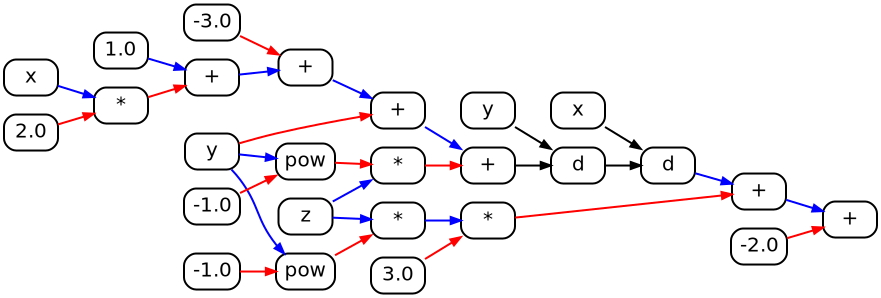
\includegraphics[scale=0.60]{../figures/dataflow.png}
    \input{dfg}
    \caption{DFG implicite construit par l'expression originale, montrée ci-dessus.}
    \label{lst:edsl}
\end{figure}\\\\

\section{Systèmes de typage}\label{sec:type-systems}

Les premiers travaux sur l'analyse dimensionnelle sans risque de type se trouvent dans \citet{kennedy1994dimension, kennedy1996programming} qui utilise les types pour coder la dimensionnalité et empêcher l'apparition de bogues courants liés à la non-concordance des dimensions, et a été réalisé plus tard dans le langage F\#~\citep{kennedy2010types}. \citet{jay1996shape}, \citet{rittri1995dimension}, et \citet{zenger1997indexed} explorent l'application des types de dimension pour l'algèbre linéaire. Plus récemment, \citet{kiselyov2005number, kiselyov2010fun} et \citet{griffioen2015type}, montrent comment manipuler des tableaux de manière plus complexe. Avec le regain d'intérêt pour l'algèbre des tenseurs et la programmation des tableaux, \citet{chen2017typesafe} et \citet{rink2018modeling} montrent comment coder la sécurité des formes pour l'algèbre des tenseurs dans divers systèmes de types.

Le problème que nous essayons de résoudre peut être résumé comme suit. Étant donné deux valeurs \inline{x} et \inline{y}, et l'opérateur \inline{\$}, comment déterminer si l'expression \inline{z = x \$ y} est valide, et si oui, quel est le type de résultat de \inline{z}? Pour la multiplication matricielle, lorsque \inline{x} $\in \mathbb{R}^{m \times n}$ et \inline{y} $\in \mathbb{R}^{n \times p}$, l'expression est bien tapée et nous pouvons déduire \inline{z} $\in \mathbb{R}^{m \times p}$. Plus généralement, nous voudrions déduire le type de \inline{z} pour un opérateur quelconque \inline{@} $ : (\mathbb{R}^\mathbf{a}, \mathbb{R}^\mathbf{b}) \rightarrow \mathbb{R}^\mathbf{c}$ où $\mathbf{a} \in \mathbb{N}^q, \mathbf{b} \in \mathbb{N}^r, \mathbf{c} \in \mathbb{N}^s$ et $q, r, s \in \mathbb{N}$. Pour de nombreuses opérations d'algèbre linéaire telles que la multiplication de matrices, $\mathcal{S}(\mathbf a, \mathbf b) \stackrel{?}{=} \mathbf c$ est calculable en $\mathcal{O}(1)$ -- on peut simplement vérifier l'équivalence des dimensions intérieures ($\mathbf{a}_2 \stackrel{?}{=} \mathbf{b}_1$).

La vérification de forme des opérateurs de tableaux multidimensionnels n'est pas toujours décidable. Pour les fonctions de forme arbitraires $\mathcal{S}(\mathbf{a}, \mathbf{b})$, la vérification $\mathcal{S}(\mathbf{a}, \mathbf{b}) \stackrel{?}{=} \mathbf{c}$ nécessite une machine de Turing. Si $\mathcal{S}$ utilise l'opérateur de multiplication, comme dans le cas de l'arithmétique convolutionnelle~\citep{dumoulin2016guide}, l'inférence de forme devient équivalente à l'arithmétique Peano, qui est indécidable~\citep{godel1931formal}. L'addition, la soustraction, l'indexation et la comparaison d'entiers sont toutes décidables en arithmétique de Presburger~\citep{suzuki1980verification, bradley2006decidable, charlier2011enumeration}. La vérification de l'égalité est trivialement décidable, et peut être mise en œuvre dans la plupart des systèmes de type statique.

L'évaluation d'un $\mathcal{S}$ arbitraire qui utilise la multiplication ou la division (par exemple, arithmétique convolutionnelle) nécessite un langage typé de manière dépendante ~\citep{xi1998eliminating, pineyro2019structure}, mais la vérification de l'égalité de forme (par exemple la vérification de forme des opérations arithmétiques ordinaires) est possible Java et ses cousins.\hspace{-.08em}\footnote{Le système de types de Java est connu pour être complet à Turing~\citep{grigore2017java}. Ainsi, l'émulation de types dépendants en Java est théoriquement possible, mais probablement insoluble en raison des limitations pratiques notées par Grigore.} De plus, nous pensons que la vérification de forme de l'arithmétique matricielle ordinaire est décidable dans tout système de type librement basé sur le système F${}_{<:}$~\citep{cardelli1991extension}. Nous proposons un système de types pour renforcer la sécurité des formes qui peut être mis en œuvre dans n'importe quel langage avec sous-typage et génériques, comme \href{https://docs.oracle.com/javase/tutorial/java/generics/index.html}{Java}~\citep{naftalin2007java}, \href{https://kotlinlang.org/docs/reference/generics.html}{Kotlin}~\citep{tate2013mixed}, \href{https://www.typescriptlang.org/docs/handbook/advanced-types.html}{TypeScript}~\citep{bierman2014understanding} ou \href{https://doc.rust-lang.org/1.7.0/book/generics.html}{Rust}~\citep{crozet2019nalgebra}.

{\tiny
    \begin{table}
        \begin{tabular}{|c||c|c|c|l|}\hline
            Math                                     &  Infix                                                                           & Prefix                                                                                    & Postfix                                                                                      & Operator Type Signature                                                                                                                                                                                      \\ \hline
            $A(B)$                                                         & \tinline{a(b)}                                                                   &                                                                                           &                                                                                              & $ (\texttt{a}:  \mathbb{R}^{\tau}\rightarrow\mathbb{R}^{\pi}, \texttt{b}: \mathbb{R}^{\lambda} \rightarrow \mathbb{R}^{\tau}) \rightarrow (\mathbb{R}^{\lambda}\rightarrow \mathbb{R}^{\pi})               $ \\ \hline
            $A\pm B$                                                       & \begin{tabular}{@{}c@{}}\tinline{a + b}\\\tinline{a - b}\end{tabular}            & \begin{tabular}{@{}c@{}}\tinline{plus(a, b)}\\\tinline{minus(a, b)}\end{tabular}          &                                                                                              & $ (\texttt{a}:  \mathbb{R}^{\tau}\rightarrow\mathbb{R}^{\pi}, \texttt{b}: \mathbb{R}^{\lambda} \rightarrow \mathbb{R}^{\pi}) \rightarrow (\mathbb{R}^{?}\rightarrow \mathbb{R}^{\pi})                      $ \\ \hline
            $A   B$                                                        & \begin{tabular}{@{}c@{}}\tinline{a * b}\\\tinline{a.times(b)}\end{tabular}       & \tinline{times(a, b)}                                                                     &                                                                                              & $ (\texttt{a}: \mathbb{R}^{\tau}\rightarrow\mathbb{R}^{m \times n}, \texttt{b}: \mathbb{R}^{\lambda}\rightarrow\mathbb{R}^{n \times p})    \rightarrow (\mathbb{R}^{?}\rightarrow\mathbb{R}^{m \times p})  $ \\ \hline
            \begin{tabular}{@{}c@{}}$\frac{A}{B}$\\$AB^{-1}$\end{tabular}  & \begin{tabular}{@{}c@{}}\tinline{a / b}\\\tinline{a.div(b)}\end{tabular}         & \tinline{div(a, b)}                                                                       &                                                                                              & $ (\texttt{a}: \mathbb{R}^{\tau}\rightarrow\mathbb{R}^{m \times n}, \texttt{b}: \mathbb{R}^{\lambda}\rightarrow\mathbb{R}^{p \times n}) \rightarrow (\mathbb{R}^{?}\rightarrow\mathbb{R}^{m \times p})     $ \\ \hline
            $\pm A$                                                        &                                                                                  & \begin{tabular}{@{}c@{}}\tinline{-a}\\\tinline{+a}\end{tabular}                           & \begin{tabular}{@{}c@{}}\tinline{a.unaryMinus()}\\\tinline{a.unaryPlus()}\end{tabular}       & $                   (\texttt{a}: \mathbb{R}^{\tau}\rightarrow\mathbb{R}^{\pi}) \rightarrow (\mathbb{R}^{\tau}\rightarrow\mathbb{R}^{\pi})                                                                  $ \\ \hline
%\begin{tabular}{@{}c@{}}sin(a)\\cos(a)\\tan(a)\end{tabular}               &                                                                                  & \begin{tabular}{@{}c@{}}\tinline{sin(a)}\\\tinline{cos(a)}\\\tinline{tan(a)}\end{tabular} & \begin{tabular}{@{}c@{}}\tinline{a.sin()}\\\tinline{a.cos()}\\\tinline{a.tan()}\end{tabular} & $                                            (\texttt{a}: \mathbb{R}\rightarrow\mathbb{R}) \rightarrow (\mathbb{R}\rightarrow\mathbb{R})                                                                   $ \\ \hline
            $\ln(A)$                                                       &                                                                                  & \begin{tabular}{@{}c@{}}\tinline{ln(a)}\\\tinline{log(a)}\end{tabular}                    & \begin{tabular}{@{}c@{}}\tinline{a.ln()}\\\tinline{a.log()}\end{tabular}                     & $                  (\texttt{a}: \mathbb{R}^{\tau}\rightarrow\mathbb{R}^{m \times m}) \rightarrow (\mathbb{R}^{\tau}\rightarrow\mathbb{R}^{m \times m})                                                     $ \\ \hline
            $\log_b A$                                                     & \tinline{a.log(b)}                                                               & \tinline{log(a, b)}                                                                       &                                                                                              & $       (\texttt{a}: \mathbb{R}^{\tau}\rightarrow\mathbb{R}^{m \times m}, \texttt{b}: \mathbb{R}^{\lambda}\rightarrow\mathbb{R}^{m \times m}) \rightarrow (\mathbb{R}^{?}\rightarrow\mathbb{R})            $ \\ \hline
            $A^{b}$                                                        & \tinline{a.pow(b)}                                                               & \tinline{pow(a, b)}                                                                       &                                                                                              & $       (\texttt{a}: \mathbb{R}^{\tau}\rightarrow\mathbb{R}^{m \times m}, \texttt{b}: \mathbb{R}^{\lambda}\rightarrow\mathbb{R}) \rightarrow (\mathbb{R}^{?}\rightarrow\mathbb{R}^{m \times m})            $ \\ \hline
            \begin{tabular}{@{}c@{}}$\sqrt{a}$\\$\sqrt[3]{a}$\end{tabular} & \begin{tabular}{@{}c@{}}\tinline{a.pow(1.0/2)}\\\tinline{a.root(3)}\end{tabular} & \begin{tabular}{@{}c@{}}\tinline{a.pow(1.0/2)}\\\tinline{a.root(3)}\end{tabular}          & \begin{tabular}{@{}c@{}}\tinline{a.sqrt()}\\\tinline{a.cbrt()}\end{tabular}                  & $                        (\texttt{a}: \mathbb{R}^{\tau}\rightarrow\mathbb{R}^{m \times m}) \rightarrow (\mathbb{R}\rightarrow\mathbb{R}^{m \times m})                                                      $ \\ \hline
            \begin{tabular}{@{}c@{}}$\frac{da}{db}$\\$a'(b)$\end{tabular}  & \tinline{a.d(b)}                                                                 & \tinline{grad(a)[b]}                                                                      & \tinline{d(a) / d(b)}                                                                        & $         (\texttt{a}: \mathbb{R}^{\tau}\rightarrow\mathbb{R}^{\pi}, \texttt{b}: \mathbb{R}^{\lambda}\rightarrow\mathbb{R}^{\omega}) \rightarrow (\mathbb{R}^{?}\rightarrow\mathbb{R}^{\pi \times \omega}) $ \\ \hline
        \end{tabular}
        \caption{\label{tab:shape_system}Kotlin$\nabla$ spécifie la forme de sortie pour les expressions tensorielles.}
    \end{table}
}
%$\dagger$ \inline{a} et \inline{b} sont des fonctions d'ordre supérieur. Il peut s'agir de constantes (par exemple 0, 1.0), de variables (par exemple \inline{Var("x")}) ou d'expressions (par exemple \inline{x + 1}, \inline{2 * x + y}).

{\small
\begin{table}[]
    \begin{tabular}{|c|c|c|c|}\hline
        Forme & $\mathbb{R}^{?}\rightarrow\mathbb{R}$ & $\mathbb{R}^{?}\rightarrow\mathbb{R}^{m}$ & $\mathbb{R}^{?}\rightarrow\mathbb{R}^{j \times k}$ \\\hline
    $\mathbb{R}^{?}\rightarrow\mathbb{R}$ & $\mathbb{R}^{?}\rightarrow\mathbb{R}$ & $\mathbb{R}^{?}\rightarrow\mathbb{R}^{m}$ & $\mathbb{R}^{?}\rightarrow\mathbb{R}^{j \times k}$ \\\hline
    $\mathbb{R}^{?}\rightarrow\mathbb{R}^{n}$ & $\mathbb{R}^{?}\rightarrow\mathbb{R}^{n}$  & $\mathbb{R}^{?}\rightarrow\mathbb{R}^{m \times n}$  &  \\\hline
    $\mathbb{R}^{?}\rightarrow\mathbb{R}^{h \times i}$ & $\mathbb{R}^{?}\rightarrow\mathbb{R}^{h \times i}$  &  &\\\hline
    \end{tabular}
    \caption{\label{tab:ho_deriv}La forme d'une dérivée du tenseur dépend de la forme de la fonction en cours de différentiation et de la forme de la variable par rapport à laquelle nous nous différencions.}
\end{table}
}

\section{Sécurité de la forme}\label{sec:shape-safety}

\noindent Il existe trois grandes stratégies pour traiter les erreurs de forme dans la programmation des tableaux:
%
\begin{enumerate}
    \item Cacher l'erreur en remodelant implicitement ou \href{https://docs.scipy.org/doc/numpy-1.15.0/user/basics.broadcasting.html}{broadcasting arrays}.
    \item Annoncer l'erreur au moment de l'exécution, par exemple: ~\href{https://www.tensorflow.org/api_docs/python/tf/errors/InvalidArgumentError}{\inline{InvalidArgumentError}}.
    \item Ne pas autoriser la compilation de programmes pouvant entraîner une erreur de forme. \\
\end{enumerate}
%
La plupart des bibliothèques de programmation de tableaux telles que NumPy~\citep{van2011numpy} ou TensorFlow~\citep{abadi2016tensorflow} utilisent la première ou la deuxième stratégie. Dans Kotlin$\nabla$, nous adoptons la troisième, qui permet à un vérificateur de type incrémental, comme ceux que l'on trouve généralement dans les EDI modernes, de détecter instantanément quand une opération de matrice est invalide. Prenons l'exemple suivant:
%
\begin{kotlinlisting}
val vecA = Vec(1.0, 2.0)      // Type inféré : Vec<Int, D2>
val vecB = Vec(1.0, 2.0, 3.0) // Type inféré : Vec<Int, D3>
val vecC = vecB + vecB
val vecD = (*@\uwave{vecA + vecB}@*) // Erreur de compilation: Expected Vec<2>, found Vec<3>
\end{kotlinlisting}
%
Tenter de faire la somme de deux vecteurs dont les formes ne correspondent pas, c'est échouer à la compilation.
%
\begin{kotlinlisting}
val matA = Mat1x4(1.0, 2.0, 3.0, 4.0) // Type inféré: Mat<Double, D1, D4>
val matB = Mat4x1(1.0, 2.0, 3.0, 4.0) // Type inféré: Mat<Double, D4, D1>
val matC = matA * matB
val matD = (*@\uwave{matA *\ matC}@*) // Erreur de compilation: Expected <4, *>, found Mat<1, 1>
\end{kotlinlisting}
%
De même, la multiplication de deux matrices dont les dimensions intérieures ne correspondent pas ne permet pas de compiler.
%
\begin{kotlinlisting}
val matA = Mat2x4(1.0, 2.0, 3.0, 4.0,
                  5.0, 6.0, 7.0, 8.0)
val matB = Mat4x2(1.0, 2.0,
                  3.0, 4.0,
                  5.0, 6.0,
                  7.0, 8.0)
val matC: Mat<Double, D2, D2> = a * b // Les types sont facultatifs, mais encouragés
val matD = Mat2x1(1.0, 2.0)
val matE = matC * matD
val matF = Mat3x1(1.0, 2.0, 3.0)
val matG = (*@\uwave{matE *\ matF}@*) // Erreur de compilation: Expected Mat<1, *>, found Mat<3, 1>
\end{kotlinlisting}
%
Il est nécessaire de spécifier les types de paramètres dans une signature de méthode. Les types de retour explicites sont facultatifs mais sont encouragés pour des raisons de lisibilité. S'ils sont omis, le système de types peut souvent les déduire:
%
\begin{kotlinlisting}
fun someMatFun(m: Mat<Double, D3, D1>): Mat<Double, D3, D3> = ...
fun someMatFun(m: Mat<Double, D2, D2>) = ...
\end{kotlinlisting}
%
La sécurité des formes est actuellement prise en charge jusqu'aux tenseurs de rang 2, c'est-à-dire les matrices. Pour effectuer la vérification des dimensions dans notre système de types, nous énumérons d'abord une liste de types littéraux entiers comme une chaîne de sous-types, $C < : C - 1 < : C - 2 < : \dots < : 1 < : 0$, où $C$ est la plus grande dimension de longueur fixe que nous souhaitons représenter, qui peut être spécifiée par l'utilisateur avant la compilation. Cela garantit une complexité linéaire dans l'espace et le temps pour le contrôle des sous-types, avec une limite supérieure constante.
%
\begin{kotlinlisting}[caption={Type sécurisé pour les tenseurs de rang 1, $\forall C\leq2.$}]
interface Nat<T: D0> { val i: Int }
// Les valeurs Int ont été réifiées pour permettre de les comparer à l'exécution
sealed class D0(open val i: Int = 0) { companion object: D0(), Nat<D0> }
sealed class D1(override val i: Int = 1): D0(i) { companion object: D1(), Nat<D1> }
sealed class D2(override val i: Int = 2): D1(i) { companion object: D2(), Nat<D2> }
sealed class D3(override val i: Int = 3): D2(i) { companion object: D3(), Nat<D3> } //...
sealed class D99(override val i: Int = 99): D98(i) { companion object: D99(), Nat<D99> }
\end{kotlinlisting}
%
Ensuite, nous surchargeons l'opérateur d'appel pour émuler l'instanciation d'une collection littérale, en utilisant l'arité pour en déduire la dimensionnalité. Considérons le cas du rang 1 pour l'inférence de longueur sur des littéraux vectoriels:
%
\begin{kotlinlisting}
open class Vec<E, Len: D1> constructor(val contents: List<E>) {
    companion object {
        operator fun <T> invoke(t: T): Vec<T, D1> = Vec(listOf(t))
        operator fun <T> invoke(t0: T, t1: T): Vec<T, D2> = Vec(listOf(t0, t1))
        operator fun <T> invoke(t0: T, t1: T, t2: T): Vec<T, D3> = Vec(listOf(t0, t1, t2))
    }
}
\end{kotlinlisting}
%
Enfin, nous surchargeons les opérateurs arithmétiques en utilisant des contraintes de forme génériques. Comme nos entiers de niveau type sont une chaîne de sous-types, nous n'avons besoin de définir qu'un seul opérateur et pouvons compter sur la substitution de Liskov~\citep{liskov1987} pour préserver la sécurité des formes pour tous les sous-types.
%
\begin{kotlinlisting}
// <C: D1> acceptera 1 <= C <= 99 via la substitution Liskov
operator fun <E, C: D1, V: Vec<X, C>> V.plus(v: V): V = TODO()
\end{kotlinlisting}
%
L'opérateur \inline{+} peut maintenant être utilisé comme tel. Les opérandes incompatibles entraîneront une erreur de frappe:
%
\begin{kotlinlisting}
// Ajout de vecteur à type contrôlé avec inférence de forme
val Y = Vec(0, 0) + Vec(0, 0) // Y: Vec<Float, D2>
val X = (*@\uwave{Vec(0, 0) + Vec(0, 0, 0)}@*) // Erreur de compilation: Vec<Int, D2>, Vec<Int, D3>
\end{kotlinlisting}
%
La construction dynamique de la longueur est également autorisée, bien qu'elle puisse échouer lors de l'exécution. Par exemple, la construction dynamique de la longueur est autorisée, bien qu'elle puisse échouer en cours d'exécution:
%
\begin{kotlinlisting}
val one = Vec(0, 0, 0) + Vec(0, 0, 0) // Fonctionne toujours en toute sécurité
val add = Vec(0, 0, 0) + Vec<Int, D3>(listOf(...)) // Se compile, mais peut échouer à l'exécution
val vec = Vec(0, 0, 0) // Type inféré : Vec<3>
val sum = (*@\uwave{Vec(0, 0) + add}@*) // Erreur de compilation: Vec<Int attendu, D2>, Vec<Int trouvé, D3>
\end{kotlinlisting}
%
Les matrices et les tenseurs ont une syntaxe similaire. Par exemple, Kotlin$\nabla$ peut déduire la forme de la multiplication de la matrice, et ne compilera pas si les dimensions internes des arguments sont en désaccord:
%
\begin{kotlinlisting}
open class Mat<X, R: D1, C: D1>(vararg val rows: Vec<X, C>)
fun <X> Mat1x2(d0: X, d1: X): Mat<X, D1, D2> = Mat(Vec(d0, d1))
fun <X> Mat2x1(d0: X, d1: X): Mat<X, D2, D1> = Mat(Vec(d0), Vec(d1))

operator fun <X, Q: D1, R: D1, S: D1> Mat<X, Q, R>.times(m: Mat<X, R, S>): Mat<X, Q, S> =
    Mt( *(rows.indices).map { i -> /* ... */ }.toTypedArray() )

val matM = Mat1x2(0, 0)
val matO = (*@\uwave{matM *\ matM}@*) // Erreur de compilation: Expected Mat<2, *>, found Mat<1, 2>
\end{kotlinlisting}
%
Une technique similaire peut être trouvée dans nalgebra~\citep{crozet2019nalgebra}, une bibliothèque d'algèbre linéaire à forme vérifiée pour le langage Rust qui utilise également des entiers synthétiques de niveau type. Cette technique trouve son origine dans Haskell, un langage qui prend en charge des formes plus puissantes de calcul au niveau des types, telles que \textit{arithmétique des types}~\citep{kiselyov2005number}. L'arithmétique des types simplifie la concaténation des tableaux, l'arithmétique convolutionnelle~\citep{dumoulin2016guide} et d'autres opérations qui sont actuellement difficiles à exprimer dans Kotlin$\nabla$, où des fonctions arbitraires de niveau type $\mathcal{S}(\mathbf a, \mathbf b)$ (ref.~\autoref{sec:type-systems}) peuvent nécessiter l'énumération de fonctions Kotlin allant jusqu'à $C^{q + r}$ pour effectuer le calcul.

\section{Test logiciel}\label{sec:testing}

Kotlin$\nabla$ prétend éliminer certaines erreurs d'exécution, mais comment savoir si la mise en œuvre n'est pas incorrecte? Une méthode est connue sous le nom de test basé sur les propriétés (PBT)~\citep{fink1997property} (\autoref{subsec:property-based-testing}), étroitement lié à la notion de test de métamorphose~\citep{chen1998metamorphic} (\autoref{subsec:metamorphic-testing}). Parmi les mises en œuvre notables, citons \href{http://www.cse.chalmers.se/~rjmh/QuickCheck/manual.html}{QuickCheck}~\citep{claessen2011quickcheck}, \href{https://hypothesis.readthedocs.io/en/latest/}{Hypothesis}~\citep{Hypothesis} et \href{https://github.com/kotlintest/kotlintest}{KotlinTest}~\citep{kotlintest}, sur lesquels notre suite de tests est basée. PBT utilise des propriétés algébriques pour vérifier le résultat d'un calcul en construisant des expressions sémantiquement équivalentes mais syntaxiquement distinctes. Lorsqu'elles sont évaluées sur les mêmes entrées, elles doivent produire la même réponse, avec une précision numérique. Deux de ces équivalences sont utilisées pour tester Kotlin$\nabla$: \\
%
\begin{enumerate}
\item \textbf{Différenciation analytique} : différencier manuellement des fonctions sélectionnées et comparer le résultat numérique de l'évaluation d'entrées choisies au hasard dans leur domaine avec le résultat numérique obtenu en évaluant la DA sur les mêmes entrées.
\item \textbf{Approximation par différence finie} : échantillonner l'espace des fonctions symboliques différentiables, en comparant les résultats numériques suggérés par la \hyperref[sec:fdm]{méthode par différence finie} et le résultat équivalent de la DA, jusqu'à une approximation de précision fixe. \\
\end{enumerate}
%
Par exemple, le test suivant vérifie si la dérivée analytique et la dérivée automatique, lorsqu'elles sont évaluées à des points aléatoires, sont égales avec une précision numérique:
%
\begin{kotlinlisting}
val z = y * (sin(x * y) - x)            // Fonction à l'essai
val dz_dx = d(z) / d(x)                 // Dérivé automatique
val manualDx = y * (cos(x * y) * y - 1) // Dérivé manuel

"dz/dx devrait être y * (cos(x * y) * y - 1)" {
    NumericalGenerator.assertAll { x0, y0 ->
    // Evaluer les résultats à une graine donnée
    val autoEval = dz_dx(x to x0, y to y0)
        val manualEval = manualDx(x to x0, y to y0)
        autoEval shouldBeApproximately manualEval // Fails iff eps < |adEval - manualEval|
    }
}
\end{kotlinlisting}
%
PBT va rechercher dans l'espace de saisie deux valeurs numériques \inline{x0} et \inline{y0}, qui violent la spécification, puis les "rétrécir" pour découvrir des valeurs limites de type "pass-fail". Nous pouvons construire un test similaire en utilisant la \hyperref[sec:fdm]{méthode des différences finies}, par exemple $f'(x)=\lim _{h\to 0}{\frac {f(x+h)-f(x)}{h}}$:
%
\begin{kotlinlisting}
val dx = 1E-8
val f = sin(x)
val df_dx = d(f) / d(x)
val fd_dx = (sin(x + dx) - sin(x)) / dx

"d(sin x)/dx devrait être (sin(x + dx) - sin(x)) / dx" {
    NumericalGenerator.assertAll { x0 ->
    val autoEval = df_dx(x0)
        val fdEval = fd_dx(x0)
        autoEval shouldBeApproximately fdEval // Fails iff eps < |adEval - fdEval|
    }
}
\end{kotlinlisting}
%
Pour plus de détails sur le PBT, voir \autoref{subsec:property-based-testing}. Il existe de nombreuses autres façons de vérifier indépendamment le gradient numérique, comme les nombres doubles ou la dérivée d'étape complexe~\citep{martins2003complex}. Une autre stratégie consiste à comparer avec un cadre AD bien connu, tel que TensorFlow~\citep{abadi2016tensorflow} ou PyTorch~\citep{paszke2019pytorch}. Dans les travaux futurs, nous avons l'intention de procéder à une comparaison plus approfondie de la précision et des performances numériques.

\section{Surcharge de l'opérateur}\label{sec:operator-overloading}

La surcharge de l'opérateur \noindent~\citep{corliss1993operator} est l'un des moyens les plus simples de mettre en œuvre la différentiation automatique. Nous utilisons la fonctionnalité \href{https://kotlinlang.org/docs/reference/operator-overloading.html}{surcharge de l'opérateur} de Kotlin sur une tour numérique (ref. ~\autoref{sec:numeric-tower}) pour fournir une notation concise pour les opérations algébriques abstraites. Par exemple, supposons que nous ayons une interface \inline{Group}, qui surcharge les opérateurs \inline{+} et \inline{*}:
%
\begin{kotlinlisting}
interface Group<T: Group<T>> {
    operator fun plus(addend: T): T
    operator fun times(multiplicand: T): T
}
\end{kotlinlisting}
%
Ici, nous spécifions un type récursif lié en utilisant une méthode connue sous le nom de polymorphisme lié à F~\citep{canning1989f} pour s'assurer que les opérations renvoient la valeur concrète de la variable de type \inline{T}, plutôt que quelque chose de plus abstrait comme \inline{Group} (en fait, \inline{T} est un type \inline{self}). Imaginez une classe \inline{Fun} qui a implémenté \inline{Group}. Elle peut être utilisée comme suit:
%
\begin{kotlinlisting}
fun <T: Group<T>> cubed(t: T): T = t * t * t
fun <X: Fun<X>> twiceExprCubed(e: X): X = cubed(e) + cubed(e)
\end{kotlinlisting}
%
Comme \href{https://docs.python.org/3/reference/datamodel.html#special-method-names}{Python}, Kotlin supporte la surcharge d'un ensemble limité d'opérateurs, qui sont évalués en utilisant un \href{https://kotlinlang.org/docs/reference/grammar.html#precedence}{précédent fixe}. Dans la version actuelle de Kotlin$\nabla$, les opérateurs n'effectuent aucun calcul, ils construisent simplement un graphe acyclique dirigé (\autoref{lst:edsl}) représentant l'expression symbolique. Les expressions ne sont évaluées que lorsqu'elles sont invoquées sous forme de fonction.

\section{Fonctions de première classe}\label{sec:first-class-functions}

En soutenant les fonctions d'ordre supérieur et les lambdas, Kotlin traite les fonctions comme des citoyens de première classe. Cela nous permet de représenter des fonctions mathématiques et des fonctions de programmation avec les mêmes abstractions sous-jacentes (c'est-à-dire des FP typés). Suite à un certain nombre d'articles récents sur les fonctions AD~\citep{pearlmutter2008reverse,wang2018backpropagation}, toutes les expressions de Kotlin$\nabla$ sont traitées comme des fonctions. Par exemple:

\begin{kotlinlisting}
fun <T: Group<T>> makePoly(x: Var<T>, y: Var<T>) = x * y + y * y + x * x
val f = makePoly(x, y)
val z = f(1.0, 2.0) // Returns a value
\end{kotlinlisting}
%
Actuellement, il est possible de représenter des fonctions où toutes les entrées et sorties partagent un seul type de données. Il peut être possible d'étendre le soutien à la création de fonctions avec différents types d'entrées/sorties et d'appliquer des contraintes sur les deux, en utilisant des limites de type covariantes et contravariantes.

\section{Tour numérique}\label{sec:numeric-tower}

Kotlin$\nabla$ utilise une tour numérique~\citep{st2012typing}. Un premier exemple de ce schéma se trouve dans \href{https://www.gnu.org/software/guile/manual/html_node/Numerical-Tower.html}{Scheme}~\citep{sperber2009revised}. Cette stratégie est également adaptée aux langages orientés objet~\citep{niculescu2003design, niculescu2011using, kennedy2005generalized} et appliquée dans des bibliothèques telles que \href{https://github.com/mipt-npm/kmath}{KMath}~\citep{nozik2019kmath} et \href{https://commons.apache.org/proper/commons-math/}{Apache Commons Math}~\citep{developers2012apache}.

\begin{kotlinlisting}
interface Group<X: Group<X>> {
    operator fun unaryMinus(): X
    operator fun plus(addend: X): X
    operator fun minus(subtrahend: X): X = this + -subtrahend
    operator fun times(multiplicand: X): X
}

interface Field<X: Field<X>> : Group<X> {
    val e: X
    val one: X
    val zero: X
    operator fun div(divisor: X): X = this * divisor.pow(-one)
    infix fun pow(exp: X): X
    fun ln(): X
}
\end{kotlinlisting}
%
La tour numérique nous permet de définir des comportements communs tels que la soustraction et la division sur des structures algébriques abstraites, par exemple \inline{Group}, \inline{Ring}, et \inline{Field}. Ces abstractions sont extensibles à des systèmes de nombres concrets, tels que les nombres complexes et les quaternions. Par exemple, pour définir plus tard un champ sur des nombres complexes ou des quaternions,\hspace{-.08em}\footnote{ex. Afin de calculer les dérivées dans un réseau de neurones à quaternions. \citep{isokawa2003quaternion}}, il faut simplement étendre la tour numérique et passer outre l'implémentation par défaut. La plupart des opérations mathématiques peuvent être définies en utilisant un petit ensemble d'opérateurs primitifs, qui peuvent être différenciés de manière générique, plutôt que sur une base ad hoc.

\section{Types de données algébriques}\label{sec:adts}

\noindent Types de données algébriques (ADT) sous forme de \href{https://kotlinlang.org/docs/reference/sealed-classes.html}{classe scellée} (alias types de somme) facilitent une forme limitée de filtrage sur un ensemble fermé de sous-classes. Lors de la comparaison avec les sous-classes d'une classe scellée, le compilateur oblige l'auteur à fournir un flux de contrôle exhaustif sur tous les sous-types concrets d'une classe abstraite. Considérons les classes suivantes:
%
\begin{kotlinlisting}
class Const<T: Fun<T>>(val number: Number) : Fun<T>()
class Sum<T: Fun<T>>(val left: Fun<T>, val right: Fun<T>) : Fun<T>()
class Prod<T: Fun<T>>(val left: Fun<T>, val right: Fun<T>) : Fun<T>()
class Var<T: Fun<T>> : Fun<T>() { override val variables: Set<Var<X>> = setOf(this) }
class Zero<T: Fun<T>> : Const<T>(0.0)
class One<T: Fun<T>> : Const<T>(1.0)
\end{kotlinlisting}
%
Lorsqu'on passe au type de classe scellée, les consommateurs doivent explicitement traiter chaque cas, car un flux de contrôle incomplet ne se compilera pas au lieu d'échouer silencieusement au moment de l'exécution. Considérons maintenant une définition simplifiée de \inline{Fun}, une classe scellée qui définit le comportement de l'invocation et de la différentiation des fonctions, en utilisant une forme restreinte de correspondance de motifs. Elle peut être construite avec un ensemble de \inline{Var}s, et peut être invoquée avec une valeur numérique:
%
\begin{kotlinlisting}
sealed class Fun<X: Fun<X>>(open val variables: Set<Var<X>> = emptySet()) : Group<Fun<X>> {
    constructor(vararg fns: Fun<X>): this(fns.flatMap { it.variables }.toSet())
    // Les sous-classes de Fun sont un ensemble fermé, aucun `else -> ...` n'est requis.
    operator fun invoke(map: Map<Var<X>, X>): Fun<X> = when (this) {
        is Const -> this
        is Var -> map.getOrElse(this) { this } // Une application partielle est autorisée
        is Prod -> left(map) * right(map) // Le casting intelligent lance implicitement après vérification
        is Sum -> left(map) + right(map)
    }

    fun d(variable: Var<X>): Fun<X> = when(this) {
        is Const -> Zero
        is Var -> if (variable == this) One else Zero
        // Règle du produit: d(u*v)/dx = du/dx * v + u * dv/dx
        is Prod -> left.d(variable) * right + left * right.d(variable)
        is Sum -> left.d(variable) + right.d(variable)
    }

    operator fun plus(addend: Fun<T>) = Sum(this, addend)
    operator fun times(multiplicand: Fun<T>) = Prod(this, multiplicand)
}
\end{kotlinlisting}
%
Le \href{https://kotlinlang.org/docs/reference/typecasts.html#smart-casts}{coulée intelligente} de Kotlin est un exemple d'analyse de type sensible au flux~\citep{pearce2011implementing} où le type abstrait \inline{Fun} peut être traité comme \inline{Sum} après avoir effectué une vérification \inline{is Sum}. Sans le smart casting, il faudrait écrire \inline{(this as Sum).left} pour accéder au membre, \inline{left}, créant une \inline{ClassCastException} potentielle si le casting se trompait.

\section{Répartition multiple}\label{sec:multiple-dispatch}

En conjonction avec les ADT, Kotlin$\nabla$ utilise l'envoi multiple pour instancier le type de résultat le plus spécifique d'une opération arithmétique en fonction du type de ses opérandes. Bien que Kotlin ne prenne pas directement en charge la répartition multiple, il peut être émulé en utilisant la répartition unique comme décrit par \citet{leavens1998multiple}. En se basant sur \autoref{sec:adts}, supposons que nous souhaitions réécrire une expression algébrique, par exemple pour réduire le gonflement de l'expression ou améliorer la stabilité numérique. Nous pouvons utiliser \inline{when} pour bifurquer sur le type d'une sous-expression au moment de l'exécution:

\begin{kotlinlisting}
override fun times(multiplicand: Fun<X>): Fun<X> =
    when {
        this == zero -> this
        this == one -> multiplicand
        multiplicand == one -> this
        multiplicand == zero -> multiplicand
        this == multiplicand -> pow(two)
        // Sans smart cast: Const((this as Const).number * (multiplicand as Const).number)
        this is Const && multiplicand is Const -> Const(number * multiplicand.number)
        // Simplification supplémentaire est possible grâce aux règles de remplacement
        else -> Prod(this, multiplicand)
    }

val result = Const(2.0) * Sum(Var(2.0), Const(3.0))
//         = Sum(Prod(Const(2.0), Var(2.0)), Const(6.0))
\end{kotlinlisting}
%
La répartition multiple nous permet de mettre tous les flux de contrôle connexes sur une seule classe abstraite qui est héritée par des sous-classes, ce qui simplifie la lisibilité, le débogage et le remaniement.

\section{Fonctions d'extension}\label{sec:extension-functions}

\href{https://kotlinlang.org/docs/reference/extensions.html}{Fonctions d'extension} permet d'augmenter les classes externes avec de nouveaux champs et méthodes. En utilisant la programmation orientée vers le contexte~\citep{hirschfeld2008context}, nous pouvons exposer des extensions personnalisées (par exemple, par le biais de \inline{DoubleContext}) aux consommateurs sans avoir besoin de sous-classement ou d'héritage.
%
\begin{kotlinlisting}[caption={We can provide numerical extensions, wrapped in a context.}]
object DoubleContext {
    operator fun Number.times(expr: Fun<Double>) = Const(toDouble()) * expr
}
\end{kotlinlisting}
%
Maintenant, nous pouvons utiliser le contexte pour définir une autre extension, \inline{Fun.multiplyByTwo()}, qui calcule le produit à l'intérieur d'un \inline{DoubleContext}, en utilisant la surcharge d'opérateur définie ci-dessus:
%
\begin{kotlinlisting}
fun Fun<Double>.multiplyByTwo() = with(DoubleContext) { 2 * this }
\end{kotlinlisting}
%
Des extensions peuvent également être définies dans un autre fichier ou contexte et importées à la demande, une approche empruntée à \href{https://github.com/mipt-npm/kmath}{KMath}~\citep{nozik2019kmath}, une autre bibliothèque mathématique pour Kotlin. Cette approche convient également à la définition de méthodes de commodité pour l'affectation de variables et d'adaptateurs de type pour les primitives numériques, en tenant compte du contexte. Par exemple:
%
\begin{kotlinlisting}
object DoubleContext: Proto<DConst, Double>() {
    override val Const<DConst, Number>.value: Double
    get() = c.toDouble()
    override fun wrap(default: Number): DConst = DConst(default.toDouble())
    override val X: X<DConst> = object: X<DConst>(DConst(0.0)) {
        override fun invoke(X: XBnd<DConst>): DConst = X.const
        override fun toString() = "X"
    }
    override val Y: Y<DConst> = object: Y<DConst>(DConst(0.0)) {
        override fun invoke(Y: YBnd<DConst>): DConst = Y.const
        override fun toString() = "Y"
    }
    override infix fun X<DConst>.to(c: Double) = XBnd(DConst(c))
    override infix fun Y<DConst>.to(c: Double) = YBnd(DConst(c))
}
\end{kotlinlisting}
%
Cette DSL, qui est utilisée pour prendre en charge la capture et le curry de variables, peut être utilisée comme suit:
%
\begin{kotlinlisting}
with(DoubleContext) {
    val t = X + Y + 0.0
    val l = t(X to 1.0, Y to 2.0) * t(X to 1.0)(Y to 3.0) // Currying
    val p = t(X to 1.0) // Partial application
    val k = (*@\uwave{t(Z to 4.0)}@*) // Does not compile
}
\end{kotlinlisting}

\section{Différentiation automatique et symbolique}\label{sec:ad_vs_sd}

S'inspirant de \citet{mccarthy1960recursive}, Kotlin$\nabla$ met en œuvre une différentiation symbolique, similaire à l'approche trouvée dans \citet[\S 2.56--2.58]{abelson1996structure}. Les expressions symboliques permettent une meilleure lisibilité, une plus grande précision numérique et une plus grande efficacité de calcul. Motivé par cette observation, nous mettons en œuvre des extensions vectorielles et matricielles à la différentiation scalaire telle que décrite par \citet{dwyer1948symbolic} et plus récemment \citet{laue2018computing}.

La littérature sur la DA affirme depuis longtemps que la différentiation automatique n'est pas une différentiation symbolique~\citep{baydin2015survey}. Beaucoup, y compris l'auteur de cette thèse, ont soupçonné cette affirmation d'être trompeuse. Récemment, cette affirmation a été mise en doute~\citep{wang2018demystifying} et réfutée~\citep{laue2019equivalence}. S'il est vrai que certaines implémentations de la différentiation automatique entrelacent l'évaluation numérique et la différentiation symbolique au moment de l'exécution, cet entrelacement n'est certainement pas une condition préalable pour qu'une bibliothèque de différentiation soit considérée comme \textit{automatique}. De même, comme le suggère la littérature antérieure~\citep{baydin2014ad}, le problème du gonflement de l'expression n'est pas unique à la différentiation symbolique~\citep{laue2019equivalence}.

La distinction entre AD et SD devient de plus en plus floue lorsque l'on considère les modèles d'exécution plus flexibles~\citep{wang2018demystifying} et les AD hybrides~\citep{abadi2016tensorflow} qui sont capables d'une évaluation à la fois enthousiaste~\citep{paszke2019pytorch, agrawal2019tensorflow} et paresseuse~\citep{neubig2017dynet, van2018tangent}. Nous estimons au contraire que la différentiation symbolique est un type de différentiation automatique que la littérature sur la DA a trop vite écarté. SD, en particulier, offre au compilateur beaucoup plus de souplesse pour effectuer des optimisations globales telles que la simplification algébrique~\citep{bergstra2010theano}, la vectorisation en boucle~\citep{agarwal2019static} et la compréhension du tenseur~\citep{vasilache2018tensor, laue2020simple}. Ces optimisations seraient autrement impossibles si leur différentiation symbolique et leur évaluation numérique étaient effectuées en synchronisme, alors que le graphique de flux de données n'est que partiellement disponible.

\section{Coroutines}\label{sec:coroutines}

Les coroutines sont une généralisation des sous-routines pour le multitâche non préventif, généralement mises en œuvre à l'aide de continuations~\citep{haynes1984continuations}. Les continuations sont un mécanisme qui permet aux fonctions d'accéder et de modifier les calculs ultérieurs. Dans le style des continuations~\citep{sussman1975scheme} (CPS), chaque fonction, en plus de ses arguments habituels, prend une autre fonction représentant la routine suivante. Plutôt que de retourner à son interlocuteur après l'achèvement, la fonction invoque sa continuation, et le processus est relancé.

Une forme de continuation, connue sous le nom de "continuations délimitées", suffit pour mettre en œuvre la DA en mode inverse avec surcharge de l'opérateur uniquement (sans structures de données supplémentaires) comme décrit par \citet{wang2018demystifying} et plus tard dans \citet{wang2018backpropagation}. Alors que les rappels dans Kotlin sont par défaut à un seul coup, les continuations délimitées réentrantes ou "à plusieurs coups" peuvent également être \href{https://gist.github.com/elizarov/ddee47f927dda500dc493e945128d661}{implémentées} à l'aide de \href{https://kotlinlang.org/docs/reference/coroutines-overview.html}{Kotlin Coroutines}. Les continuations délimitées "multi-shot" simplifieraient grandement notre mise en œuvre de la DA, permettraient un ensemble plus souple de primitives pour la programmation asynchrone et méritent d'être étudiées plus avant.

\section{Comparaison}\label{sec:comparison}

Inspiré par \href{https://github.com/Functional-AutoDiff/STALINGRAD}{Stalin$\nabla$}~\citep{pearlmutter2008using}, \href{https://github.com/HIPS/autograd/}{Autograd}~\citep{maclaurin2015autograd, maclaurin2016phd}, \href{http://deeplearning. net/software/theano/}{Theano}~\citep{bergstra2010theano}, \href{https://github.com/mila-iqia/myia}{Myia}~\citep{breuleux2017automatic, vanmerrienboer2018ad}, \href{https://github. com/uniker9/JAutoDiff/}{JAutoDiff}~\citep{nureki2012jautodiff}, \href{https://tongfei.me/nexus/}{Nexus}~\citep{chen2017typesafe}, \href{https://feiwang3311.github.io/Lantern/}{Lanterne}~\citep{wang2018demystifying}, \href{https://github. com/google/tangent}{Tangent}~\citep{van2018tangent}, \citet{elliott2018simple}, \href{https://people.csail.mit.edu/tzumao/gradient_halide/}{Halide}~\citep{li2018halide} et al, Kotlin$\nabla$ tente de transposer les récents développements en matière de différentiation automatique (AD) à la langue Kotlin. Ce faisant, il introduit un certain nombre d'idées expérimentales, notamment \hyperref[sec:shape-safety]{compile-time shape-safety}, \hyperref[sec:multiple-dispatch]{algebraic simplification} et la vérification de la stabilité numérique par \hyperref[sec:testing]{property-based testing}. Travaux antérieurs, notamment \href{https://pytorch.org/}{PyTorch}~\citep{paszke2019pytorch}, \href{https://www.tensorflow.org/}{TensorFlow}~\citep{abadi2016tensorflow}, \href{https://chainer. org/}{Chainer}~\citep{chainer}, \href{https://deeplearning4j.org/}{DL4J}~\cite{team2016dl4j} et d'autres ont développé des bibliothèques AD d'usage général dans des langues moins sûres.

Contrairement à la plupart des implémentations existantes, Kotlin$\nabla$ est un AD purement symbolique, basé sur des graphes, qui ne nécessite pas de métaprogrammation de modèles, d'augmentation de la puissance du compilateur ou de réflexion sur l'exécution. Comme nous l'avons vu, cette approche est principalement réalisée par \hyperref[sec:operator-overloading]{surcharge d'opérateur}, polymorphisme paramétrique et \hyperref[sec:adts]{correspondance de modèles}. L'avantage pratique de cette technique est qu'elle peut être mise en œuvre sous la forme d'une simple bibliothèque ou d'un langage intégré spécifique au domaine (eDSL), ce qui permet d'exploiter le système de types du langage hôte pour recevoir gratuitement la complétion de code et l'inférence de type. Notre approche utilise plusieurs idiomes fonctionnels, notamment les expressions lambda, les fonctions d'ordre supérieur, l'application partielle, le curry et les types de données algébriques. Pour une comparaison détaillée de Kotlin$\nabla$ avec les bibliothèques AD existantes, voir \autoref{tab:ad_comparison}.\\

\begin{table}
    \begin{tabular}{llllllllll}
        Cadriciel & Langage &
        \rot{Différenciation symbolique} &
        \rot{Différenciation automatique} &
        \rot{Programmation différentiable} &
        \rot{Programmation fonctionnelle} &
        \rot{Type sécurisé} &
        \rot{Forme sécurisée} &
        \rot{Type dépendant} &
        \rot{Multi plateforme}
        \\ \hline
        \href{https://github.com/breandan/kotlingrad}{Kotlin$\nabla$}                    & Kotlin  & \cmark & \cmark & \cmark & \cmark & \cmark & \cmark & \xmark & \wmark \\
        \href{https://diffsharp.github.io/DiffSharp/}{DiffSharp}                          & F\#     & \xmark & \cmark & \cmark & \cmark & \cmark & \xmark & \xmark & \xmark \\
        \href{https://github.com/fsprojects/fsharp-ai-tools}{TensorFlow.FSharp}          & F\#     & \xmark & \cmark & \cmark & \cmark & \cmark & \cmark & \xmark & \xmark \\
%\href{https://github.com/ThoughtWorksInc/DeepLearning.scala}{DeepLearning.scala} & Scala   & \xmark & \cmark & \cmark & \cmark & \cmark & \xmark & \xmark & \xmark \\
        \href{https://tongfei.me/nexus/}{Nexus}                                          & Scala   & \xmark & \cmark & \cmark & \cmark & \cmark & \cmark & \xmark & \xmark \\
        \href{https://feiwang3311.github.io/Lantern/}{Lantern}                           & Scala   & \xmark & \cmark & \cmark & \cmark & \cmark & \xmark & \xmark & \xmark \\
%\href{https://github.com/HuwCampbell/grenade}{Grenade}                           & Haskell & \xmark & \cmark & \xmark & \cmark & \cmark & \cmark & \xmark & \xmark \\
        \href{https://github.com/leopiney/tensor-safe}{Tensor Safe}                      & Haskell & \xmark & \cmark & \xmark & \cmark & \cmark & \cmark & \cmark & \xmark \\
        \href{https://github.com/hasktorch/hasktorch}{Hasktorch}                         & Haskell & \xmark & \cmark & \cmark & \cmark & \cmark & \cmark & \xmark & \xmark \\
        \href{https://deeplearning4j.org}{Eclipse DL4J}                                  & Java    & \xmark & \cmark & \xmark & \xmark & \cmark & \xmark & \xmark & \xmark \\
        \href{https://uniker9.github.io/JAutoDiff/}{JAutoDiff}                            & Java    & \cmark & \cmark & \cmark & \xmark & \cmark & \xmark & \xmark & \xmark \\
%\href{https://halide-lang.org}{Halide}                                           & C++     & \xmark & \cmark & \cmark & \xmark & \cmark & \xmark & \xmark & \xmark \\
        \href{https://github.com/Functional-AutoDiff/STALINGRAD}{Stalin$\nabla$}         & Scheme  & \xmark & \cmark & \cmark & \xmark & \xmark & \xmark & \xmark & \xmark \\
        \href{https://github.com/mila-iqia/myia}{Myia}                                   & Python  & \cmark & \cmark & \cmark & \cmark & \xmark & \xmark & \xmark & \wmark \\
% \href{https://github.com/HIPS/autograd/}{Autograd}                               & Python  & \xmark & \cmark & \xmark & \xmark & \xmark & \xmark & \xmark & \xmark \\
        \href{https://github.com/google/jax}{JAX}                                        & Python  & \xmark & \cmark & \cmark & \cmark & \xmark & \xmark & \xmark & \wmark \\
%        \href{https://github.com/google/tangent}{Tangent}                                & Python  & \xmark & \cmark & \xmark & \xmark & \xmark & \xmark & \xmark & \xmark \\

    \end{tabular}
    \caption{\label{tab:ad_comparison} Comparaison des bibliothèques AD. Bien que nous ne fassions pas de distinction entre AD et SD comme décrit dans \autoref{sec:ad_vs_sd}, nous adoptons ici la nomenclature préférée des auteurs. Nous faisons une distinction entre les bibliothèques de programmation différentiable (\autoref{sec:differentiable-programming}) et celles qui construisent simplement des réseaux de neurones. Le symbole \wmark indique un travail en cours.}
\end{table}

Kotlin$\nabla$ préconise l'utilisation de la programmation de tableaux fonctionnels et sans danger pour les types, mais n'impose pas ses préférences aux consommateurs. Si l'utilisateur omet la forme, il revient à la vérification de la forme en cours d'exécution. Conformément à la philosophie du langage hôte, les utilisateurs peuvent utiliser leur style de programmation préféré, en introduisant progressivement des contraintes pour profiter des avantages d'une vérification de type plus forte et se prévaloir de ses caractéristiques de programmation fonctionnelle plus riches.

\section{Travaux futurs}\label{sec:future-work}

%\vspace{40pt}\setlength{\epigraphwidth}{0.80\textwidth}
%{\pigraph{``Il est bien connu que le problème central de l'ensemble des mathématiques modernes est l'étude des fonctions transcendantes définies par des équations différentielles.''}{\begin{flushright}--Felix \citet{klein1893lectures}, \textit{Lectures sur les mathématiques}\end{flushright}}

\vspace{2pt}\setlength{\epigraphwidth}{0.60\textwidth}
\epigraph{La dérivée, telle que cette notion apparaît dans le calcul différentiel élémentaire, est un exemple mathématique familier d'une fonction pour laquelle le domaine et l'intervalle sont tous deux constitués de fonctions.''}{\begin{flushright}--Alonzo \citet{church1941calculi}, \href{https://archive.org/details/AnnalsOfMathematicalStudies6ChurchAlonzoTheCalculiOfLambdaConversionPrincetonUniversityPress1941}{\textit{Les Calculs de Conversion Lambda}}\end{flushright}}

Le dérivé, tel qu'il est couramment utilisé, est généralement associé au calcul des infinitésimaux. Mais les mêmes règles de différentiation symbolique introduites par Leibniz et Newton il y a plus de trois siècles ont réapparu dans des endroits étranges et merveilleux. Dans \citet{brzozowski1964derivatives}, nous rencontrons un exemple de différentiation symbolique dans un cadre discret, c'est-à-dire des expressions régulières. Les travaux de Brzozowski ont des applications importantes et de grande portée dans la théorie des automates~\citep{berry1986regex, antimirov1996partial, champarnaud1999regular} et l'analyse incrémentale~\citep{might2011parsing, moss2014derivatives}. Plus tard, dans \citet{thayse1981boolean}, le calcul différentiel booléen a été introduit pour la première fois,\hspace{-. 08em}\footnote{\aussi les premiers travaux sur le sujet remontent à \citet{talantsev1959analysis} et \citet{sellers1968analyzing}} une branche de l'algèbre booléenne qui a des applications importantes dans la théorie de la commutation~\citep{thayse1973boolean} et la synthèse des circuits numériques~\citep{steinbach2017boolean}. La différentiation symbolique a des applications utiles dans d'autres contextes mathématiques, notamment $\lambda$-calculus~\citep{ehrhard2003differential, cai2014theory, kelly2016evolving, brunel2020backpropagation}, incremental computation~\citep{alvarez2019fixing, alvarez2019change}, théorie des types~\citep{mcbride2001derivative, mcbride2008clowns, chen2012type}, théorie des catégories~\citep{blute2006differential, blute2009cartesian}, théorie des domaines~\citep{edalat2002domain}, théorie des probabilités~\citep{kac1951probability} et logique linéaire~\citep{ehrhard2018introduction, clift2018derivatives}.

De nombreux autres exemples de différentiation symbolique peuvent être trouvés dans des corps de littérature sans rapport. Ces indices semblent suggérer une connexion non réalisée entre la géométrie différentielle et algébrique, ce qui pourrait apporter des idées importantes pour la programmation différentiable et l'étude de la propagation des changements sur les graphiques de calcul.

Les travaux décrits dans ce chapitre établissent un cadre pour l'exploration de la différentiation symbolique à l'aide de structures algébriques comme \inline{Group}, \inline{Ring}, et \inline{Field} (\autoref{sec:numeric-tower}). Dans nos travaux futurs, nous espérons explorer la relation entre la programmation différentiable et la différentiation symbolique dans d'autres topologies. Il existe peut-être un mécanisme analogue à la descente de gradient qui peut être exploité pour accélérer l'optimisation dans de tels espaces, par exemple pour l'apprentissage des variables booléennes et d'autres structures de données comme les graphiques et les arbres.

Comme le montrent les ouvrages précédents~\citep{bergstra2010theano, baydin2015survey, laue2019equivalence}, la houle d'expression intermédiaire est un problème pernicieux en algèbre informatique et en différentiation automatique. La procédure de simplification algébrique ad hoc décrite dans \autoref{sec:multiple-dispatch} est presque certainement inadéquate pour les cas d'utilisation générale. Une direction intéressante serait de former un modèle pour minimiser la dérive numérique, en appliquant des règles de réécriture à usage général. Il existe une longue liste de travaux antérieurs sur les algorithmes de réécriture pour la stabilité numérique, qui remonte à \citet{kahan1965summation, dekker1971floating, ogita2005accurate} et qui a été explorée plus récemment par \citet{zaremba2014learning, zaremba2016learning} et ~\citet{wang2019global} dans une perspective d'apprentissage automatique.

Fournir un type de structure matricielle (par exemple, \ \inline{Singular}, \inline{Symmetric}, \inline{Orthogonal}) permettrait des spécialisations de la dérivée de matrice (\S 2.8 of~\citet{petersen2012matrix} pour un examen détaillé des techniques spécifiques de différentiation des matrices structurées). En termes d'amélioration du système de types, \citet{makwana2018numlin} a mis au point un codage de l'algèbre linéaire par types linéaires qui serait également intéressant à explorer.

Du point de vue des performances, la migration vers un backend d'algèbre linéaire dédié tel que \href{https://deeplearning4j.org/docs/latest/nd4j-overview}{ND4J}~\citep{team2016nd4j}, \href{https://commons.apache. org/proper/commons-math/}{Apache Commons Math}~\citep{developers2012apache}, \href{http://ejml.org}{EJML}~\citep{abeles2010efficient} ou \href{http://jblas.org/}{JBlas}~\citep{braun2011jblas} permettrait probablement d'accélérer les choses. À terme, nous prévoyons de compiler vers une représentation intermédiaire dédiée telle que \href{https://docs.tvm.ai/dev/relay_intro.html}{RelayIR}~\citep{roesch2018relay} ou \href{https://www.tensorflow.org/mlir}{MLIR}~\citep{mlir} afin de recevoir une accélération matérielle sur d'autres plateformes.

\section{Épilogue}

Dans ce chapitre, nous avons fait la démonstration de Kotlin$\nabla$, un langage intégré spécifique à un domaine pour la programmation différenciée et de sa mise en œuvre dans le langage de programmation Kotlin. En utilisant notre DSL comme véhicule, nous avons exploré quelques sujets intéressants en matière de différentiation automatique et de programmation de tableaux de formes sécurisées. L'auteur souhaite remercier Hanneli Tavante, Alexander Nozik, Erik Meijer, Maxime Chevalier-Boisvert, Kiran Gopinathan, Jacob Miller et Adam Pocock pour leurs précieux commentaires durant le développement de ce projet. Pour plus d'informations sur Kotlin$\nabla$, veuillez consulter le site \url{https://github.com/breandan/kotlingrad}.
